The \emph{People} page contains a grid with all volunteers that are part of our organization.  By clicking on each contact image or name, it is possible to navigate to the person's details page. It is possible to search a person by typing the name of the desired person  through the group links above the grid. 

\subsubsection{People in-the-small}
\begin{figure}[h!]
		\centering
		\begin{minipage}[b]{1\textwidth}
    			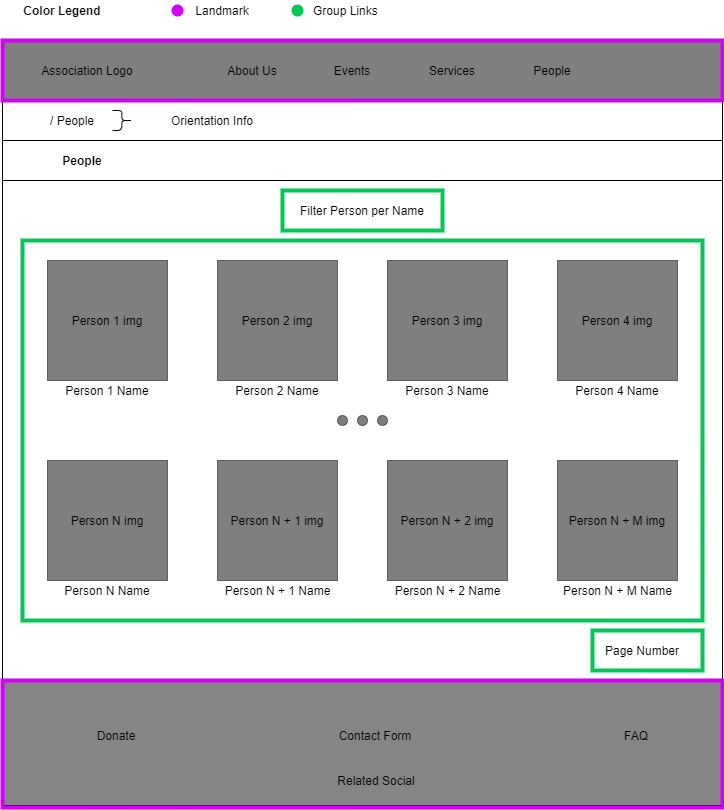
\includegraphics[width=\textwidth]{./assets/people.png}
			\caption{People Page - Design in the small.}
		\end{minipage}
	\end{figure}
	\FloatBarrier

\clearpage

\subsubsection{People screenshot}
\begin{figure}[h!]
	\centering
	\begin{minipage}[b]{1\textwidth}
    		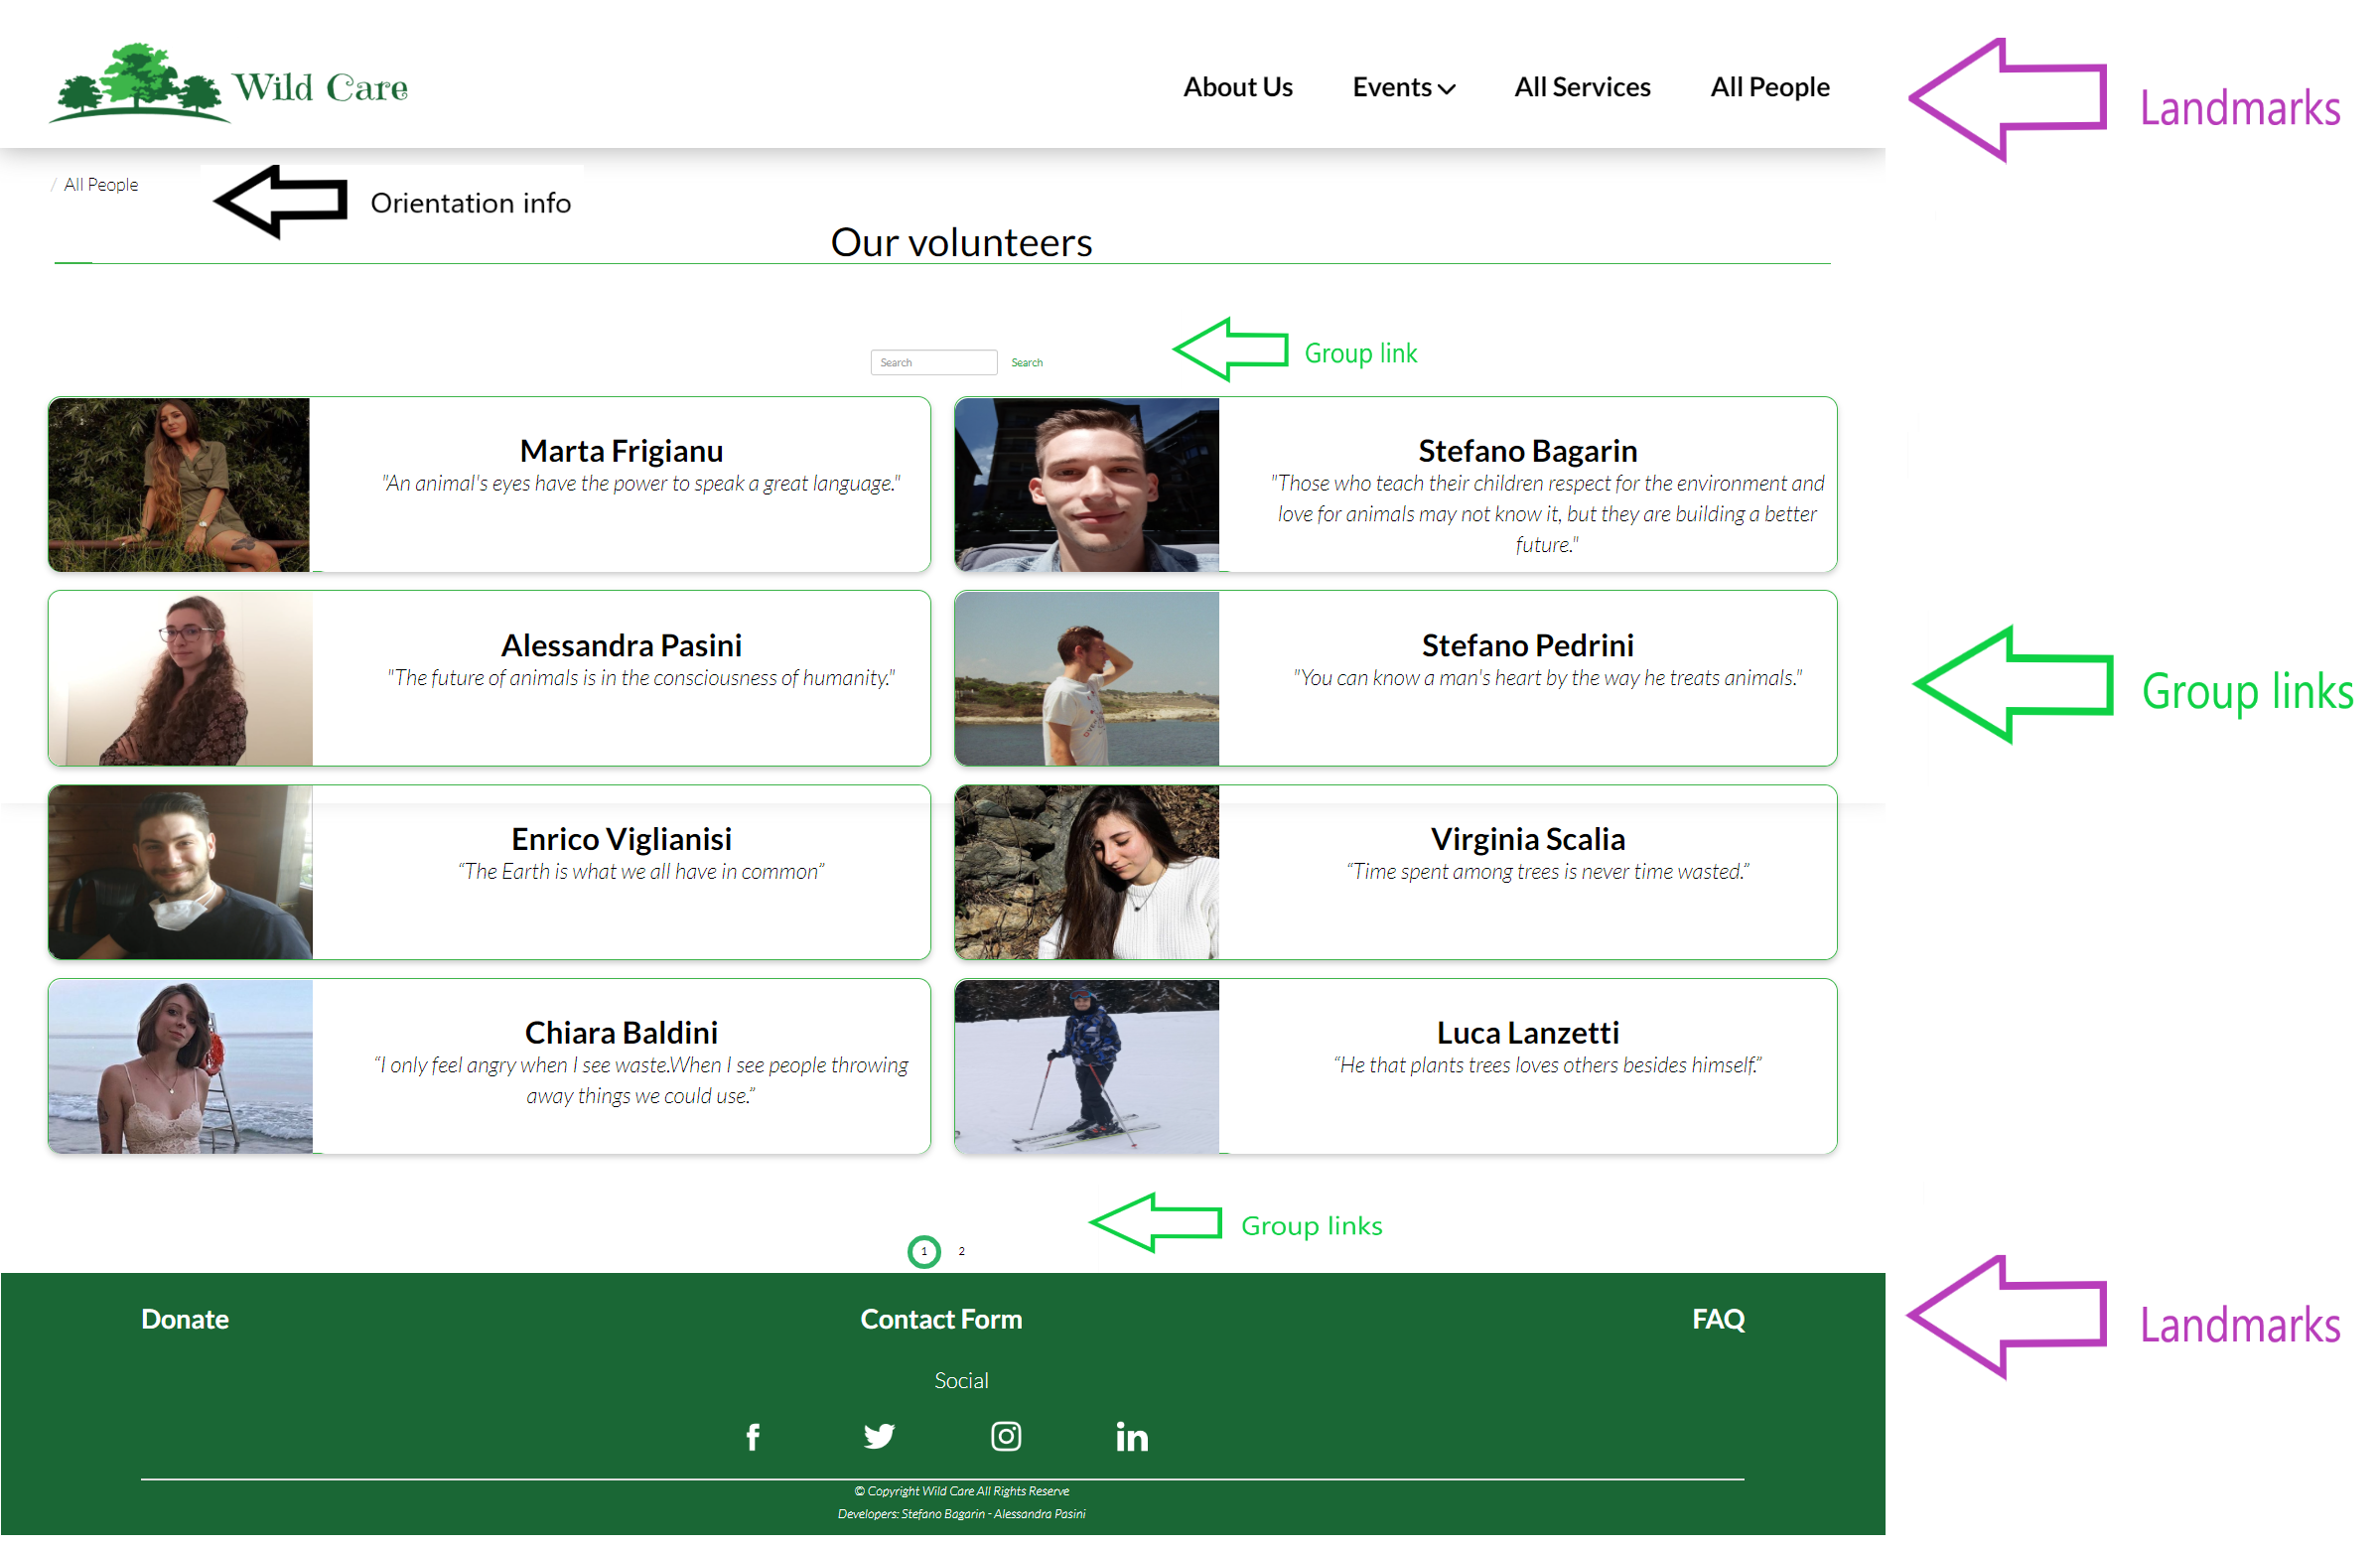
\includegraphics[width=\textwidth]{./assets/mockups/people_commented.png}
		\caption{People Page - Screenshot commented.}
	\end{minipage}
\end{figure}
\FloatBarrier

\vspace{1cm}
\hspace{-1cm}
People's details can be found in Person page, which contains:
\begin{itemize}
	\item all person's information stored into the database such as the contact image, anagraphics as name and birthday, contacts 			info as email and number,	a brief description, etc. etc.
	\item the transition links to all services the person is involved in
	\item the transition link to the events for which he/she is the point of reference. It may happen that a person doesn't have any 		transition link to events.
\end{itemize} 

\clearpage

\subsubsection{Person in-the-small}
\begin{figure}[h!]
		\centering
		\begin{minipage}[b]{1\textwidth}
    			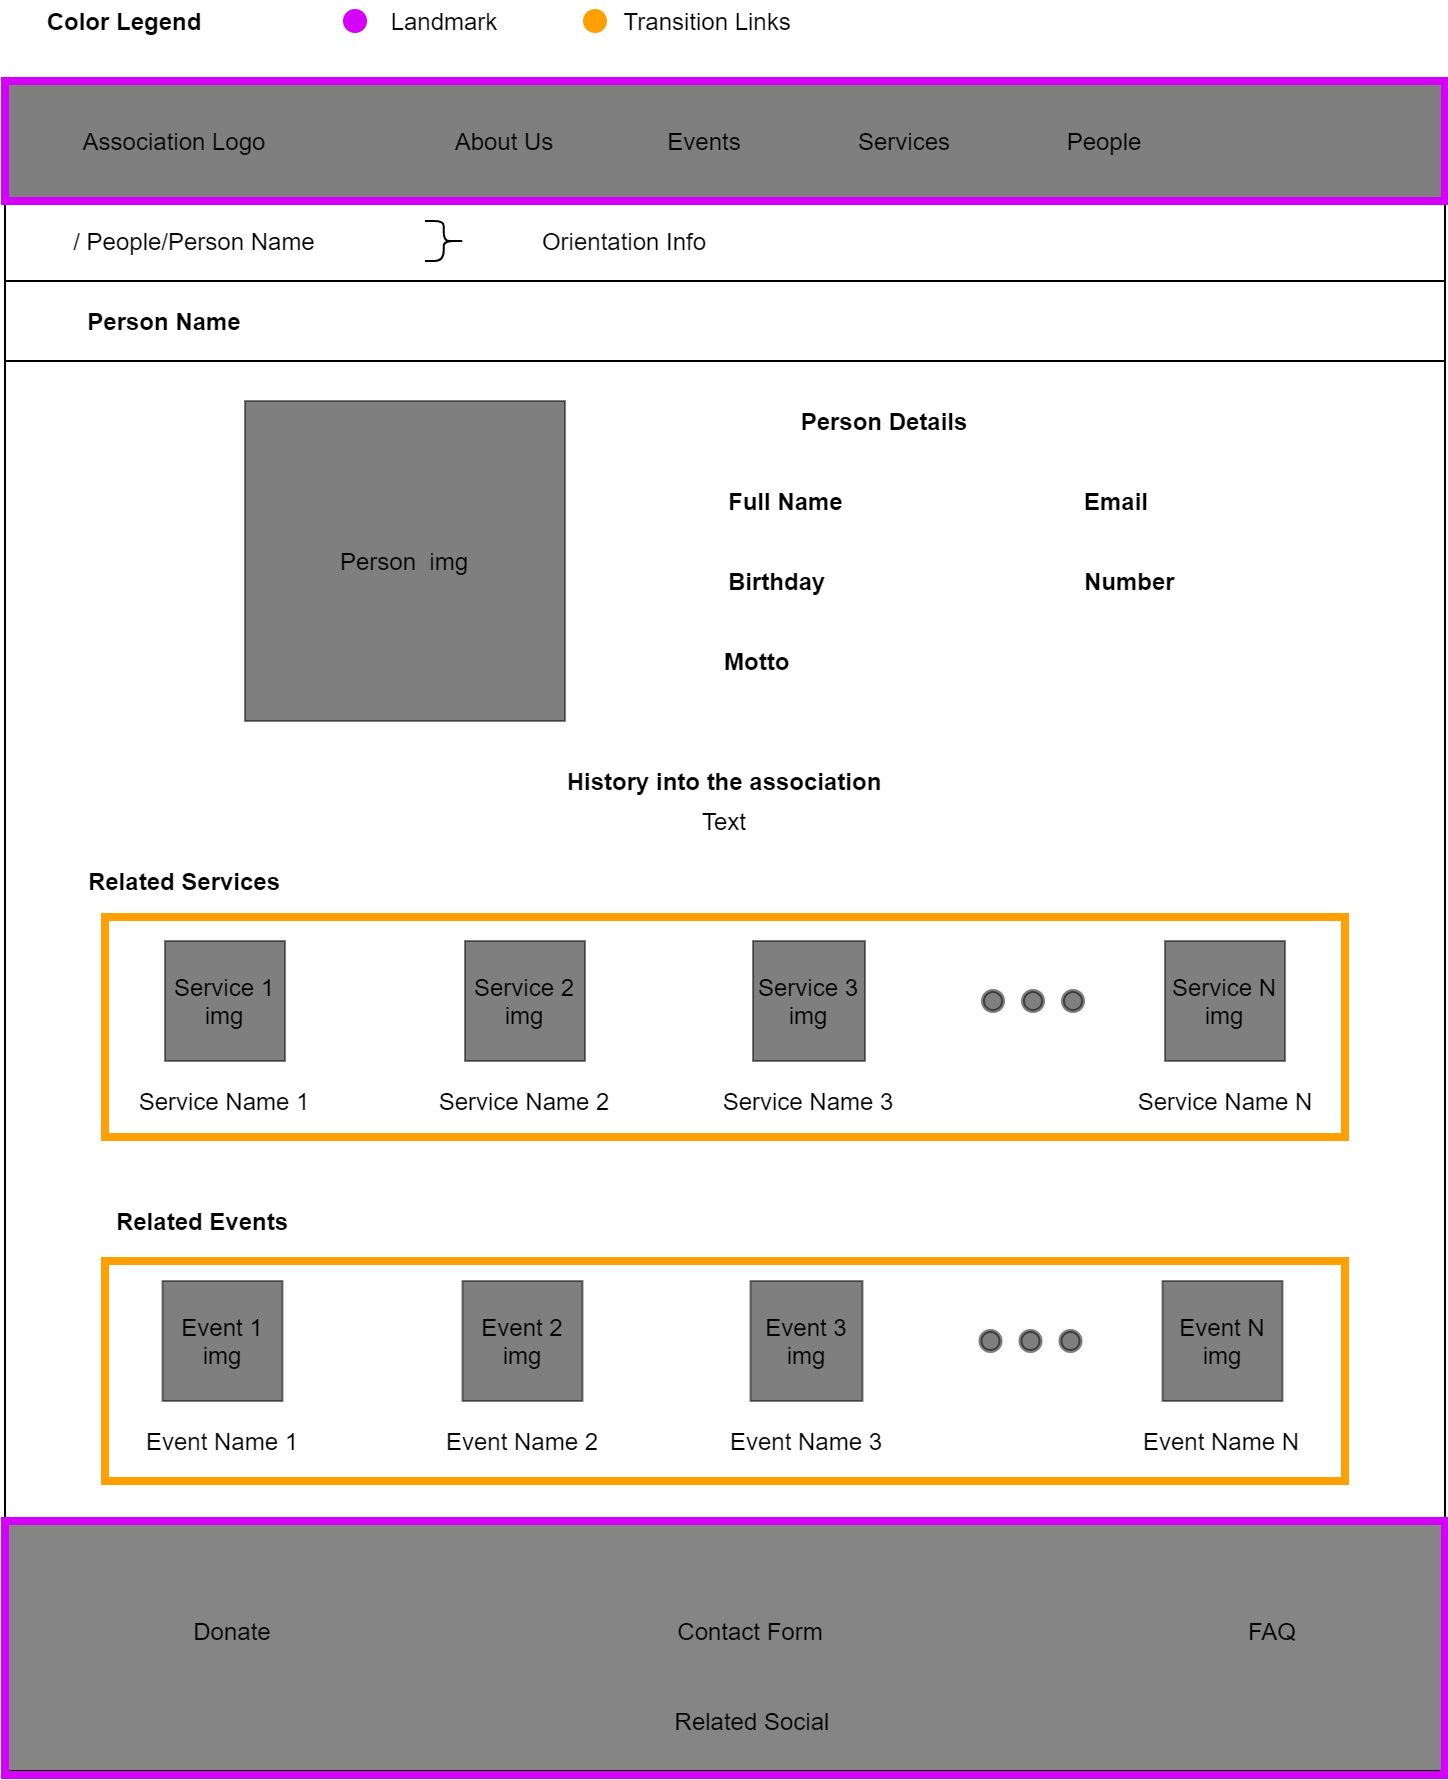
\includegraphics[width=\textwidth]{./assets/persondetails.png}
			\caption{Person Page - Design in the small.}
		\end{minipage}
\end{figure}
\FloatBarrier

\clearpage

\subsubsection{Person screenshot}
\begin{figure}[h!]
	\centering
	\begin{minipage}[b]{1\textwidth}
    		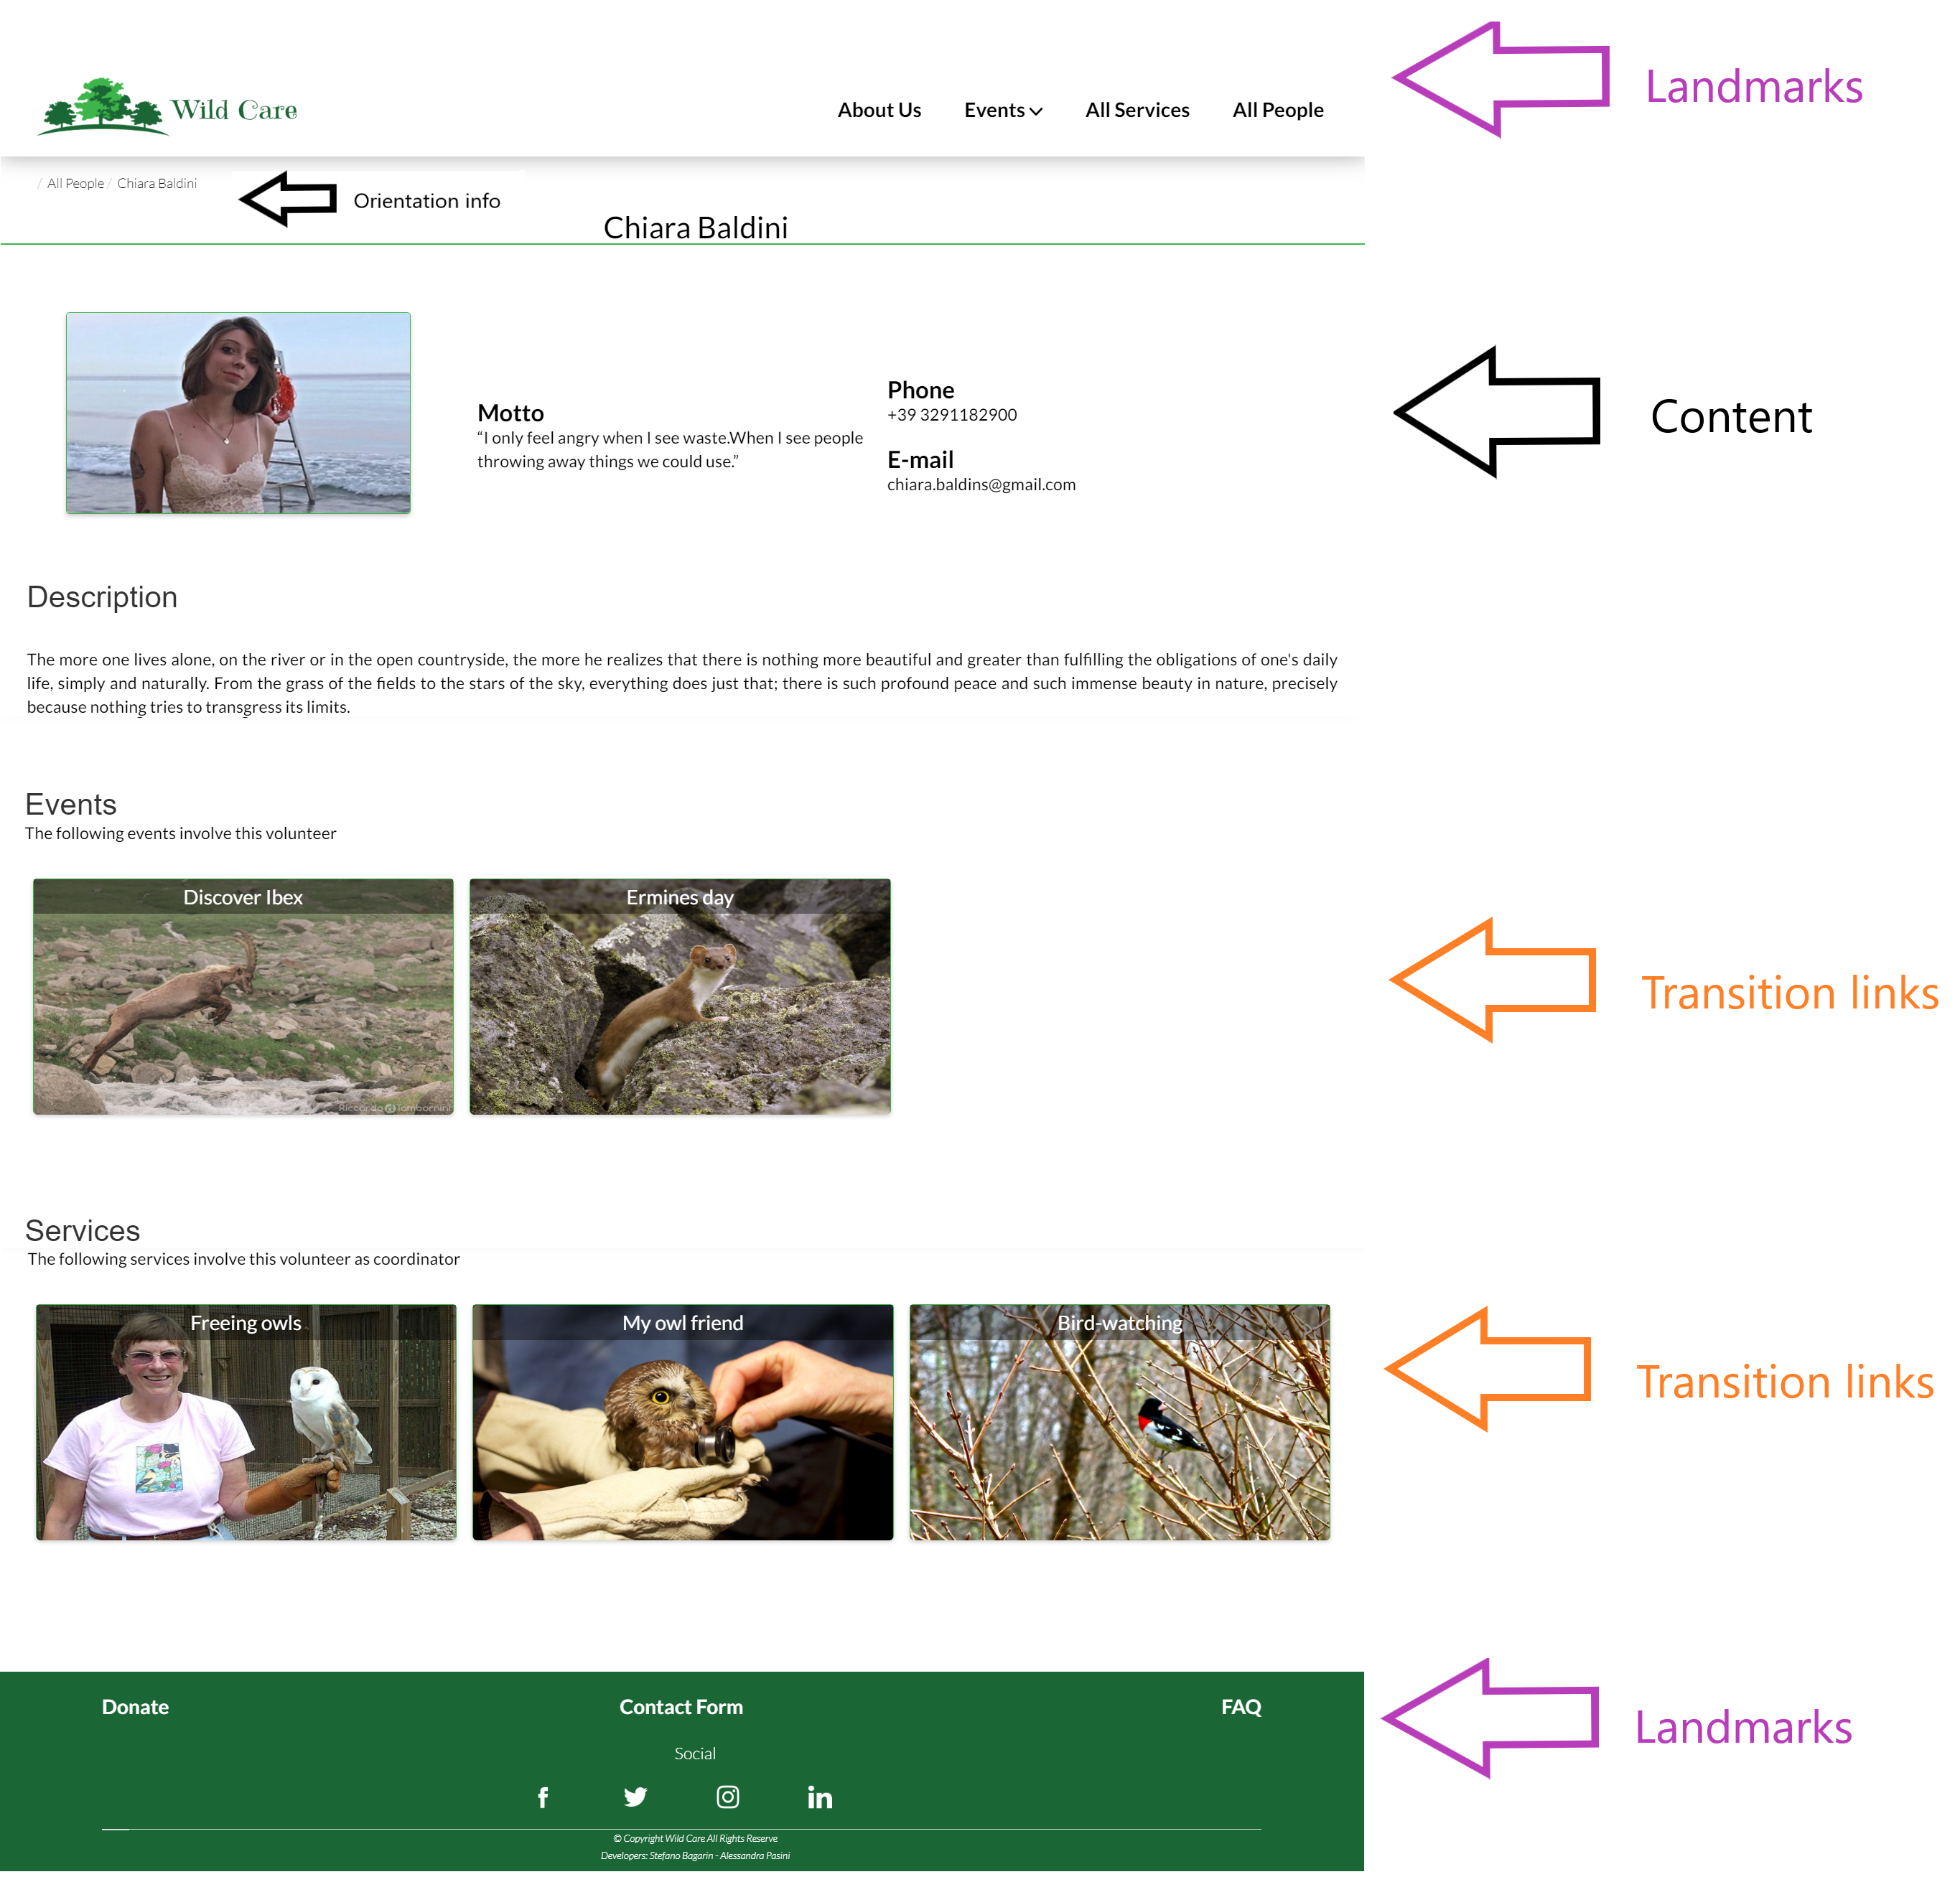
\includegraphics[width=\textwidth]{./assets/mockups/persondetails_commented.png}
		\caption{Person Page - Screenshot commented.}
	\end{minipage}
\end{figure}
\FloatBarrier
